\documentclass[a4paper,10pt]{article}
\usepackage[T1]{fontenc}
\usepackage[utf8]{inputenc}
\usepackage{lmodern}
\usepackage{url,csquotes}
\usepackage{fancyhdr}
\usepackage{graphicx}
\usepackage{epstopdf}
\usepackage{lastpage}
\usepackage{listings}
\usepackage{fancyref}
%\usepackage{subfigure}
\usepackage{enumitem}
\usepackage{tabularx, booktabs ,multirow}
\usepackage{mathtools}
\usepackage{caption}
\usepackage{subcaption}
\captionsetup{justification=centering}
\usepackage{anysize} %%pour pouvoir mettre les marges qu'on veut 
\marginsize{2cm}{2cm}{2cm}{2cm} 

\usepackage{amsfonts,amssymb,amsmath,amsthm} 
\newcommand{\vect}[2]{ $\begin{pmatrix} #1 \\  #2 \end{pmatrix} $  }

\newcommand{\matrice}[3]{ \begin{pmatrix}  #1 &  #3 \\ #3  & #2 \end{pmatrix}   }

\newcommand{\norm}[1]{\left\lVert #1 \right\rVert} 
\newcommand{\norme}[1]{\left\lVert #1 \right\rVert_2} 
\newcommand{\fsurg}{\frac{f}{g}} 
\newcommand{\prodv}[2]{ #1^T #2 } 

\usepackage{enumitem} 

% Graph package
\usepackage{tikz}
\usetikzlibrary{arrows}

\begin{document}


\begin{center}
\rule{\textwidth}{3pt}
Master MVA \\
Dynamic Programming \& Reinforcement Learning \\
TP1 - 13/11/2016 \\
\textsc{ Achari Berrada Youssef} \\
\rule{\textwidth}{.3pt}
\end{center}

\section{The On-Site Tree Cutting Problem :}
\begin{enumerate}[label=\underline{\textbf{Q\arabic*}:}]

\item The state $X$ and the action $A$ space are : 

\begin{align*}
X & = \{1, ... , \text{max\_height}, \text{sick\_state}  \} &   \\
A & = \{ 1 , 2 \} & \qquad \text{1 for keep and 2 for cut} \\
(P)_{i,j,a} = p_{i,j,a} & = \mathbb{P}(x_{t+1} = j | x_t = i , a_t = a) & \qquad  \forall (i,j) \in X^2 ,  a \in A \\ 
(R)_{i,a} = r_{i,a} &  = r(i,a) & \qquad \forall (i,a) \in X \times A
\end{align*}

The matrix $P$ of size $|X| \times |X| \times |A|$ models the random effects. 

\item \textbf{Policy Evaluation: } For a stationary policy $\pi$ : 

\[   
V^{\pi}(x)  = \mathbb{E}_{x_0 = x} \left[  \sum_{t = 0}^\infty \gamma^t r(x_t,\pi(x_t)) \right]
\]
\begin{itemize}
\item Dynamic Programming:
\begin{align*}
V^{\pi}(x) & = r(x,\pi(x)) + \gamma \sum_{y \in X} p(y | x, \pi(x)) V^{\pi}(y) \\ 
\Rightarrow & \\
V^{\pi} &  = R^{\pi} + \gamma P^{\pi} V^{\pi} \\
\Rightarrow & \\ 
V^{\pi} & = (I - \gamma P^{\pi} )^{-1} R^{\pi}
\end{align*}

\item Reinforcement Learning with Mont\'e-Carlo: In this method, we approximate the value with $N$ trajectories, and each one has $T$ steps. 
\begin{align*}
\hat{V}^{\pi} & = \frac{1}{N} \sum_{i=1}^N \, \sum_{t=0}^T \gamma^t r(x_t^i , \pi(x_t^i))
\end{align*}

\end{itemize}

\item  \textbf{Optimal Policy: } 

\begin{itemize}
\item Value Iteration: 
\begin{enumerate}[label=\arabic*.]
\item For a given initial policy $\pi_i$, we compute the Value function $V_0$ using DP or RL methods. 
\item For $k=1,..,K$,  $V_{k+1} = \mathcal{T} V_k $ with $\mathcal{T}$ is the Bellman operator. 
\item Find the Greedy policy $\pi_f$ with $\pi_f (x) = \underset{a \in A}{\text{argmax}} \, Q_K(x,a)$ \\ 
with : 
\[
Q_k(x,a) = r(x,a) + \gamma \sum_{y \in X} p(y|x,a) V^k (y) 
\]
\end{enumerate}


\item Policy Iteration: 

\begin{enumerate}[label=\arabic*.]
\item Let $\pi_0$ be the initial stationary policy,
\item For $k=0,..,K-1$, we evalute the policy $\pi_k$ and compute $V^{\pi_k}$. Then we improve the policy by finding the greedy policy $\pi_{k+1}$ with $\pi_{k+1} (x) = \underset{a \in A}{\text{argmax}} \, Q_k(x,a)$ 
\item Return $\pi_{K}$.
\end{enumerate}

\end{itemize}

\item Optimal policy: 
\begin{itemize}
\item Value iteration is computationally efficient but the convergence is asymptotic. 

\item Policy iteration converge is a small number of iterations but each iteration requires a full policy evaluation which might be expensive. 
\end{itemize}
\begin{figure}[!h]
        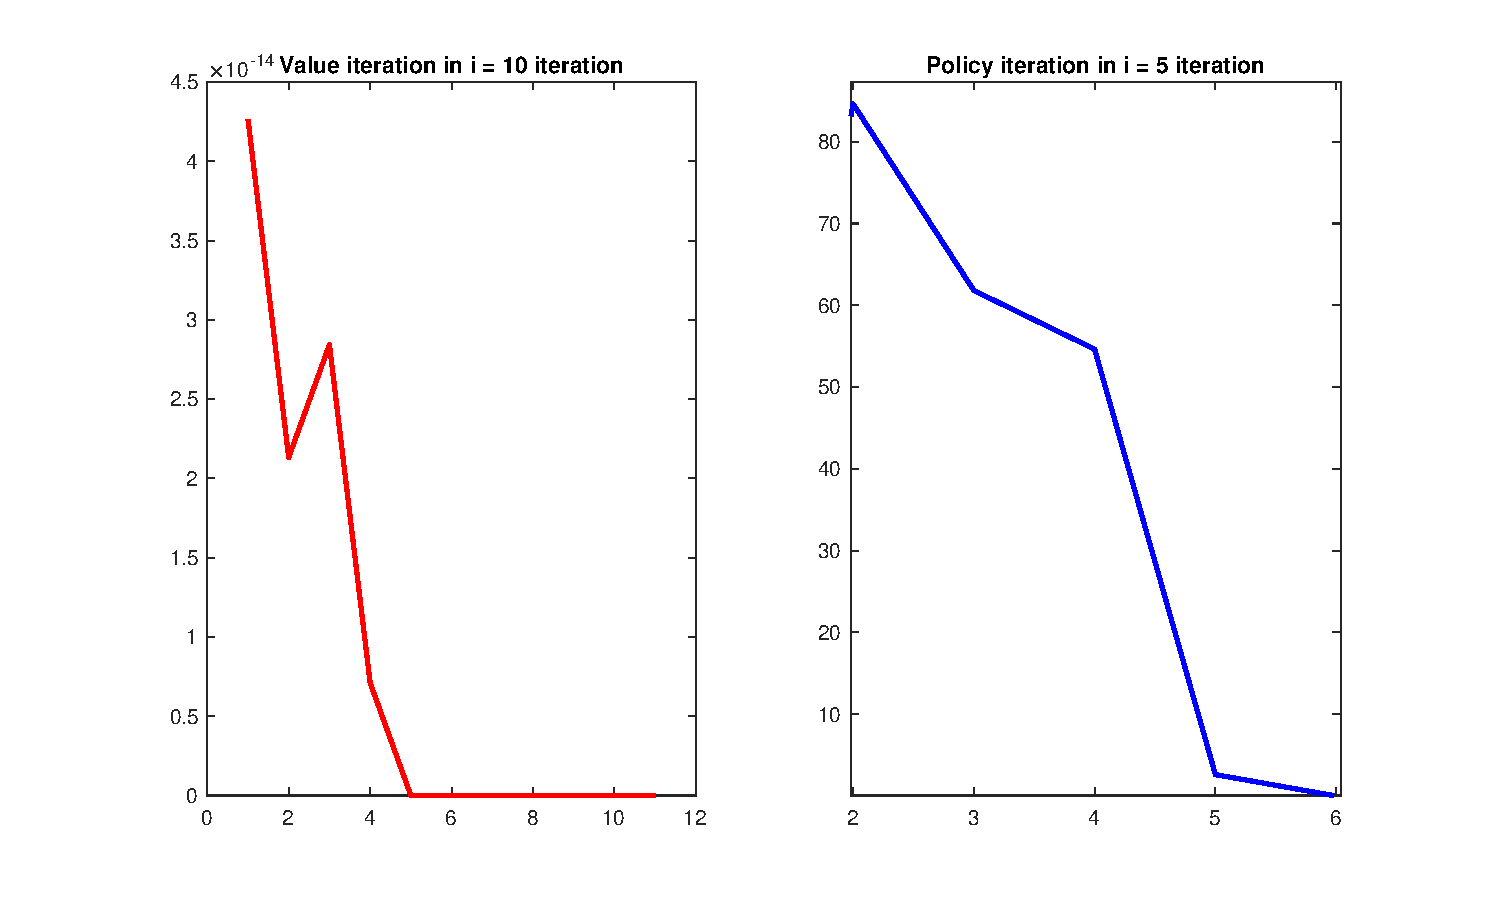
\includegraphics[width=.95\linewidth]{ValuevsPolicy.eps}  
        \caption{Value iteration error vs Policy iteration error }%\label{fig:animals}
\end{figure}

\end{enumerate}

\end{document}
